\section{Selection}
\label{sec:analysis:selection}



\subsection{Object Selection}
\label{sec:analysis:selection:object}

The event topologies of interest will require reconstructing electrons, muons, hadronically decaying tau leptons, hadronic jets, \PQb tagged jets, and missing tansverse energy (\MET or MET).  In this section, the reconstruction and selection of these physics objects is described.



\subsubsection{Primary vertex}
Primary vertices (PV) are reconstructed based on information from the tracking subsystem, mainly through the inner pixel detector. Quality cuts are applied to reconstructed PVs to guarantee they come from a proton-proton hard scattering event. These cuts are as follows,
\begin{equation*}
    N_{\rm d.o.f.}> 4; \quad  \left|z\right| < 24\cm; \quad \sqrt{x^{2} + y^{2}} < 2\cm.
\end{equation*}


\noindent The PVs are ordered based on the sum \pt of their reconstructed tracks. Selected physics objects are associated to the PV with the greatest sum \pt. 




\subsubsection{Muon}
Muon candidates are reconstructed using both the muon and tracker systems. The coverage of these two detector systems allows reconstruction of muons within $\left|\eta\right| < 2.4$ and $p_{T}$ as low as 5\GeV~\cite{Chatrchyan:2012xi}. The details of particle-flow muon reconstruction are described in Section~\ref{sec:cmsExperiment:reconstruction:muon}. In the analysis, selected muons are required to be reconstructed using both the \emph{global} muon and \emph{tracker} muon reconstruction algorithms. The former begins with tracker information and extrapolates to find consistency with hits in the muons system, while the latter inverts the reconstruction steps starting from the muon system and finding tracks that are consistent. The combination of these two algorithms makes for a muon reconstruction that is accurate in predicting muon momentum and efficient in detecting muons within the detector acceptance.

In the interest of detecting muons decaying from vector bosons, a set of identification and isolation requirements are applied~\cite{Sirunyan:2018fpa}. The muon identification requirements are designed to have high selection efficiency and a low probability of misidentifying non-prompt muons originating from non-bosonic decays. The muon POG provided selection criteria are listed in table~\ref{tab:analysis:selection:muon_id}.

\begin{table}[ht]
    \centering
    \setlength{\tabcolsep}{2em}
    \renewcommand{\arraystretch}{1.25}
    % \small
    \caption{Tight muon identification criteria as provided by muon POG}
    \label{tab:muon_id}
    \begin{tabular}{l|c}
    variable                            & cut value \\
    \hline
    isGlobal                            & True      \\
    isPF                                & True      \\
    $\chi^{2}$                          & $< 10$    \\
    number of matched stations          & $> 1$     \\
    number of pixel hits                & $> 0$     \\
    number of track layers              & $> 5$     \\
    number of valid hits                & $> 0$     \\
    $|d_{xy}|$                          & $< 0.2$   \\
    $|d_{z}|$                           & $< 0.5$    \\
    \hline
    $ISO_{PF}/p_{T}$ ($\rho$ corrected) & $< 0.15$
    \end{tabular}
\end{table}


\noindent To increase the likelihood of selecting muons produced by the prompt decay of vector bosons, an isolation requirement is placed on all muons. The isolation of the muon is calculated by summing the \pt of all charged hadronic, neutral hadronic, and photon particle flow candidates in a cone of radius $\Delta R = 0.4$ about the muon candidate. This quantity is corrected to remove the contamination of the neutral component due to pileup by subtracting off the average energy deposited by pileup. It is defined as,
\begin{equation*} 
    Iso_\mathrm{PF} = Iso_\mathrm{ ch. had} + \max\left(0, Iso_\mathrm{ neu. had} + Iso_{\gamma} - 0.5 Iso_\mathrm{ pileup}\right)\,.
\end{equation*}








\subsubsection{Electron}

Electrons are reconstructed by combining information from the electromagnetic calorimeter and the tracking system using a gaussian-sum filter (GSF) method \cite{Baffioni:2006cd}. The details of the particle-flow electron reconstruction are described in Section~\ref{sec:cmsExperiment:reconstruction:egamma}. All electrons are required to have $\pt \geq 20 \GeV$ and $|\eta| < 2.5$.  Electrons are identified using a tight cut-based scheme. The requirements for this selection are listed in table~\ref{tab:analysis:selection:electron_id}.

\begin{table}[ht]
    \centering
    \setlength{\tabcolsep}{2em}
    \renewcommand{\arraystretch}{1.25}
    % \small
    \caption{Tight electron identification criteria as provided by the egamma POG.}
    \label{tab:slt:electron_id}

    \begin{tabular}{l|c|c}
        variable                          & $|\eta| < 1.4446$ & $|\eta| \geq 1.566$ \\
        \hline
        $\sigma_{i\eta}\sigma_{i\eta}$    & $<0.00998$        & $0.0394$            \\
        $|d\eta|$                         & $<0.00308$        & $0.0292$            \\
        $|d\phi|$                         & $<0.0816$         & $0.00605$           \\
        $H/E$                             & $<0.0414$         & $0.0641$            \\
        $|\frac{1}{E} - \frac{1}{p}|$     & $<0.0129$         & $0.0129$            \\
        missing hits                      & $\leq 1$          & $\leq 1$            \\
        $|d_{0}|$                         & $<1.$             & $<1.$               \\
        \hline
        conversion rejection              & true              & true                \\
        ISO$_{PF}$/$p_{T}$ (EA corrected) & $< 0.0588$        & $<0.0571$           \\
    \end{tabular}
\end{table}

\noindent The electrons are also required to pass a tight isolation criteria. The isolation variable is constructed by summing the energy of charged and neutral particle flow objects within a cone of radius $\Delta R = 0.4$ about the electron candidate and subtracting off the contribution from pileup.  The combined particle flow isolation with the pileup correction is,
\begin{equation*}
    Iso_\mathrm{comb} = Iso_\mathrm{ ch. had.} + \max\left(0, Iso_\mathrm{ neu. had.} + Iso_{\gamma} - \rho A_\mathrm{eff}(\abs{\eta_{\Pe}}) \right)\,,
\end{equation*}
\noindent The pileup correction is dependent on the parameter $\rho$ which correlates with the average energy due to pileup, and the effective area which changes depending on the $|\eta|$ value of the electron.





\subsubsection{Hadronic Tau}

Hadronically decaying tau leptons are reconstructed using the hadron-plus-strips algorithm~\cite{ref:cms-tau}. This algorithm constructs candidates seeded by a PF jet that are consistent with either a single or triple charged pion decay of the tau lepton.  In the single charged pion decay mode, the presence of neutral pions is detected by reconstructing their photonic decays. The details of the hadronic tau identification is described in Section~\ref{sec:cmsExperiment:reconstruction:tau}. 

Reconstructed hadronic taus are required to have $p_{T} > 20\GeV$ and $|\eta| < 2.3$ unless noted otherwise.  If the hadronic tau candidate is found to overlap ($\DR < 0.3$) with either an electron or muon passing the analysis selections listed above, the tau candidate is rejected. To reduce fakes from electrons and muons that not passing the analysis selections listed above, MVA discriminators are applied, which requires VTight electron rejection working point and Tight muon rejection working point. Jets originating from non-tau decays are rejected with a MVA discriminator that takes into account the pileup contribution to the neutral component of the tau decay~\cite{CMS-TAU-16-003-001}.  It is observed that the counting analysis is more sensitive to misidentification faking by hadronic jets. So while the tight working point is used in the shape analysis, the very tight working point is used for the counting analysis. 








\subsubsection{Jet}
Jets are reconstructed from particle-flow (PF) candidates \cite{ref:pf}. PF candidates combine information from all of the detector subsystems to facilitate the reconstruction and identification of individual particles.  These PF candidates are clustered using the anti-\kt algorigthm \cite{Cacciari:2008gp} with a cone size of $\DR = 0.4$. Once reconstructed, a number of corrections are applied to the jets to correct for pileup contamination, differing absolute response in jet \pt, and relative response in $\eta$ \cite{ref:jetscale}.  To reduce contamination from photons and prompt leptons, several ID requirements are placed on the jets and are listed in table~\ref{tab:analysis:selection:jet_id_2016}.

\begin{table}[ht]
    \centering
    \setlength{\tabcolsep}{0.8em}
    \renewcommand{\arraystretch}{1.25}
    % \small
    \caption{Jet ID requirements for 2016.}
    \label{tab:slt:jet_id_2016}
    \begin{tabular}{l|ccc}
        \hline
                                    & $|\eta| < 2.4$ & $2.4 < |\eta| \leq 3.0$ & $3.0 < |\eta| \leq 4.7$ \\
        \hline                                                                   
        number of constituents         & $> 1$          & $> 1$                  & -- \\
        neutral hadronic fraction      & $< 0.99$       & $< 0.99$               & -- \\
        neutral EM fraction            & $< 0.99$       & $< 0.99$               & $<0.9$ \\
        charged hadronic fraction      & $> 0$          & --                     & -- \\
        charged EM fraction            & $< 0.99$       & --                     & -- \\
        number of charged constituents & $> 0$          & --                     & -- \\
        number of neutrals             & --             & --                     & $>10$                   \\
        \hline
    \end{tabular}
\end{table}

\noindent In addition to the above requirements, it is required that all jets have $\pt > 30\GeV$ and $|\eta| < 4.7$.  Jets are vetoed if they overlap with a muon, electron, or tau passing the identification requirements described above within a cone size of $\Delta R = 0.3$. 

\subsubsection{$\mathrm{b}$ Tag} The identification of jets originating from the decay of \PQb quarks is done using the CSV \PQb tagging algorithm~\cite{Sirunyan:2298594} is used to optimize the efficiency for identifying \PQb jets while reducing the misidentification from jets originating from light quarks. Details of the \PQb tagging algorithms are described in section~\ref{sec:cmsExperiment:reconstruction:btag}.  In this analysis, the recommended medium working point ($\text{CSV} > 0.8484$) supplied by the \PQb tag POG is used. 




\subsubsection{Summary}

Table~\ref{tab:analysis:selection:ObjectSelectionSum} gives a summary of the selection of physics objects, including electrons, muons, taus, jets and \PQb tags. The corrections and calibrations of the physics objects are described in Section~\ref{sec:analysis:calibration:objects}.


    \begin{tabular}{c|c|c|c }
    
        \hline
             & kinematic space  & reconstruction quality  & overlapping veto\\ \hline                                                                   
        \multirow{2}{*}{\Pe}    & \multirow{2}{*}{$\pt>20\GeV, ~\abs{\eta}<2.5$}    & Tight identification  &   \\
                                &                                                   & Tight isolation       &   \\ \hline
        \multirow{2}{*}{\PGm}   & \multirow{2}{*}{$\pt>10\GeV, ~\abs{\eta}<2.4$}    & Tight identification  &   \\
                                &                                                   & Tight isolation       &   \\ \hline
        \multirow{4}{*}{\PGth}  & \multirow{4}{*}{$\pt>20\GeV, ~\abs{\eta}<2.3$}    & Decay mode matching   &   \multirow{4}{*}{$\DR(\PGth,\Pe/\PGm)>0.3$} \\
                                &                                                   & (V)Tight isolation    &   \\
                                &                                                   & Tight \PGm rejection  &   \\
                                &                                                   & VTight \Pe rejection  &   \\ \hline
        jet                     & \multirow{2}{*}{$\pt>30\GeV, ~\abs{\eta}<2.5$}    & Loose identification  &   \multirow{2}{*}{$\DR(j,\Pe/\PGm/\PGth)>0.4$} \\
        (\PQb tag)              &                                                   & (Medium CSV)          &   \\                    
        \hline
    \end{tabular}





\FloatBarrier

% ===========================
% Event Selection
% ===========================
\subsection{Event Selection}
\label{sec:analysis:selection:event}

The event selection begins by requiring an event pass the lowest \pt theshold single electron or muon trigger that is not prescaled. From these datasets it is possible to select on a number of \WW-like final states originating from \ttbar and \tW production.  These final states are constructed based on the number of reconstructed leptons, jet multiplicity, and \PQb tag multiplicity.  The categorization of these events differs between the counting and shape analysis.  The common definition of the categories are listed in Table~\ref{tab:analysis:selection:event_categories}. There are eight channels defined by the multiplicities of leptons: 
\begin{itemize}
    \item \cee, \cem, \cet, \ceh channels based on single electron trigger; 
    \item \cme, \cmm, \cmt, \cmh channels based on the single muon trigger/
\end{itemize}
\noindent In addition, $n_j$ and $n_\PQb$ requirement are applied to further partition these eight channels, which are illustrated in Table~\ref{tab:analysis:selection:jet_categories}. These selections are designed to primarily target \ttbar production and specific \PW decay modes. The final states will tend to only contain events from a single datastream except for the \cem selection which has non-negligible overlap between the electron and muon datastreams. Any overlap in events between the two datastreams are removed by only taking the event from single muon datastream. The shape analysis merges \cem and \cme channel, while the counting analysis keeps the two separated, requiring additionally $\pt^\Pe  >(<) \pt^\PGm$ in \cem (\cme) if an event satisfies both channel.



\begin{table}
    \caption{Baseline categorization of events based on the triggering electron or muon, the presence of isolated reconstructed charged leptons.}
    % plus additional jets, identified or not as originating from a \PQb quark. Kinematic criteria required on the charged leptons and jets are listed in the last column. Categories without hadrons in the final state require also the selected leptons to have opposite-sign (OS) charge. %Overlap between events that are collected in both electron and muon triggered data streams is properly accounted for.
    \label{tab:analysis:selection:event_categories}
    \centering                                                              
    \renewcommand{\arraystretch}{1.8}           
    \setlength{\tabcolsep}{0.5em}
    % \resizebox{0.9\textwidth}{!}{                                           
    \begin{tabular}{c|c|ccc|c|c}     
        \hline 
        trigger                & label  & $N_{\Pe}$ & $N_{\PGm}$ & $N_{\PGt}$   & \pt & other  \\
        \hline                                                                                      
        \multirow{4}{*}{\Pe}   & \cee   & 2         & 0          & 0            & $\pt^{\Pe(\Pe)}  > 30 \, (20)\GeV$ & OS, $|m_{\cee} - m_{\PZ}| > 15\GeV$   \\
                               & \cem   & 1         & 1          & 0            & $\pt^{\Pe(\PGm)} > 30 \, (10)\GeV$ & OS\\
                               & \cet   & 1         & 0          & 1            & $\pt^{\Pe(\PGth)}> 30 \, (20)\GeV$ & OS\\
                               & \ceh   & 1         & 0          & 0            & $\pt^{\Pe} > 30\GeV$               &    \\
        \hline                                                                      
        \multirow{4}{*}{\PGm}  & \cme   & 1         & 1          & 0            & $\pt^{\PGm(\Pe)}  > 25 \, (20)\GeV$ & OS \\
                               & \cmm   & 0         & 2          & 0            & $\pt^{\PGm(\PGm)} > 25 \, (10)\GeV$ & OS,$|m_{\cmm} - m_{\PZ}| > 15\GeV$  \\
                               & \cmt   & 0         & 1          & 1            & $\pt^{\PGm(\PGth)}> 25 \, (20)\GeV$ & OS \\
                               & \cmh   & 0         & 1          & 0            & $\pt^{\PGm} > 25\GeV$               &    \\\hline 
                        
    \end{tabular}
    % }                                                          
\end{table}


\begin{table}[]
    \centering
    \setlength{\tabcolsep}{0.6em}
    \renewcommand{\arraystretch}{1.5}
    \caption{Categorization of the events with electron, muon, and/or tau leptons passing the reconstruction criteria, based on their jet and \PQb-tagged jet multiplicities. The yellow cells are the regions Incorporated in the shape analysis only. Also shape analysis splits $n_j=2$ and $n_j\geq 3$ regions for \cet and \cmt channels, shown as the yellow lines.}
    \begin{tabular}{l|c|c|c c|c}

                                    & $N_j = 0$     & $N_j = 1$      & $N_j = 2$                    & \multicolumn{1}{|c|}{$N_j = 3$}   & $N_j \geq 4$ \\
	\hline
    \multirow{2}{*}{$N_\PQb = 0$}   & \cellcolor{yellow}\cet, \cmt,  & \cellcolor{yellow}\cet, \cmt,& \multicolumn{2}{c}{\cellcolor{yellow}\cet, \cmt}      & \cellcolor{yellow}\\
                                    & \cellcolor{yellow}\cem         & \cellcolor{yellow}\cem       & \multicolumn{2}{c}{\cellcolor{yellow}\cee, \cmm, \cem}& \cellcolor{yellow}\\
	\hline
    \multirow{3}{*}{$N_\PQb = 1$}   &   & \cellcolor{yellow} \cet, \cmt, \cem  & \cet, \cmt   & \multicolumn{2}{!{\color{yellow}\vrule width 2pt}c}{\cet, \cmt} \\
	\cline{3-6}
                                    & \multicolumn{2}{c|}{} & \multicolumn{3}{c}{\cee, \cmm, \cem}                                        \\
	\cline{4-6}
                                    & \multicolumn{4}{c|}{} & \ceh, \cmh \\
	\hline

    \multirow{3}{*}{$N_\PQb \geq 2$} & \multicolumn{2}{c|}{} & \cet, \cmt & \multicolumn{2}{!{\color{yellow}\vrule width 2pt}c}{\cet, \cmt} \\
	\cline{4-6}
                                    & \multicolumn{2}{c|}{} & \multicolumn{3}{c}{$\cee, \cmm, \cem$}                                        \\
	\cline{4-6}
                                    & \multicolumn{4}{c|}{} & \ceh, \cmh \\
	\hline
    \end{tabular}
    
    \label{tab:analysis:selection:jet_categories}
\end{table}





% For the counting analysis, there is always a requirement that there be at least two jets and at least one \PQb tagged jet. The categories are partitioned based on whether there is exactly one \PQb jet or there are two or more \PQb jets. Additionally, the \cem selection is split into muon triggered and electron triggered categories: if the muon has the highest \pt and the muon trigger has fired it categorized as a \cme event; if the electron has highest \pt and the electron trigger fired it is categorized as an \cem event.


The additional subdivisions of the dataset in the shape analysis are illustrated as yellow cells and lines in Table~\ref{tab:analysis:selection:jet_categories}. These lower jet multiplicity and lower \PQb tag multiplicity regions function as control regions to constrain systematic uncertainties, thus takes some special event selection requirement than Table~\ref{tab:analysis:selection:event_categories}. As described in the list above, the \cee and \cmm categories have a \PZ veto applied in the case that there are one or more \PQb tags; this requirement is not applied in the zero \PQb tag case.  There is also a set of requirements to enhance the proportion of Drell-Yan in the \cet and \cmt categories in the case that the number of jets is zero or one and there are no \PQb tags.  The requirements are constructed to mainly reduce the \PW boson contribution and are :
\begin{equation*}
    40 \GeV \leq m_{\ell\PGt_{h}} \leq 100 \GeV, \quad \Delta\phi(\ell, \PGt_{h}) > 2.5, \quad m_{\rm T}^{\ell, MET} < 60 \GeV,
\end{equation*}

\noindent where $m_{T}^{\ell, MET} $ is the transverse mass of the electron or muon,
\begin{equation}
\label{eq:trans_mass}
    m_{T}^{\ell, MET} = \sqrt{2 \pt^{\ell}\MET (1-\cos\Delta\phi(\pt^{\ell}, \MET))}.
\end{equation}


\subsubsection{Yields and Kinematics Distributions}
For shape analysis, the yields are shown in Table~\ref{tab:analysis:selection:yieldsShape1} and \ref{tab:analysis:selection:yieldsShape2}. The kinematics distributions are included in Appendix~\ref{sec:analysis:plot:shape}. For counting analysis, the yields are shown in Table~\ref{tab:analysis:selection:yieldsCounting}. The kinematics distributions are included in Appendix~\ref{sec:analysis:plot:counting}.



\subsubsection{Leptons from Boson Decays and Tau Decays} 
Because the tau can decay to an electron, muon, or hadronically, each of these channels has some mixing between terms arising from $\PW\rightarrow\ell$ decays and $\PW\rightarrow\PGt\rightarrow\ell$ decays.  The mixing between the selected final states and the underlying \PW boson decays are shown in Table~\ref{tab:analysis:selection:signal_breakdown}. These numbers are estimated from simulated \ttbar events and are consequently dependent on the values of branching fractions used in the simulation. The expected proportions of $\PW\rightarrow\ell$ decays and $\PW\rightarrow\PGt\rightarrow\ell$ decay in the selected sample can be studied by calculating the signal-over-background ratio. For \cmm channel, the distributions of the tailing muon \pt and impact parameter are shown in Figure~\ref{fig:analysis:selection:sob_mumu_lep2_pt}. In the lower plots in Figure~\ref{fig:analysis:selection:sob_mumu_lep2_pt}, the ratios between $\ttbar/\tW \to \PGm \PGt \to \PGm \PGm$ and other simulations are shown as orange dots, while the ratios between $\ttbar/\tW \to \PGm \PGm$ and other simulations are shown as blue dots. The ratios are calculated as function of the tailing muon \pt and impact parameter.

 \begin{figure}[h]
  \centering
  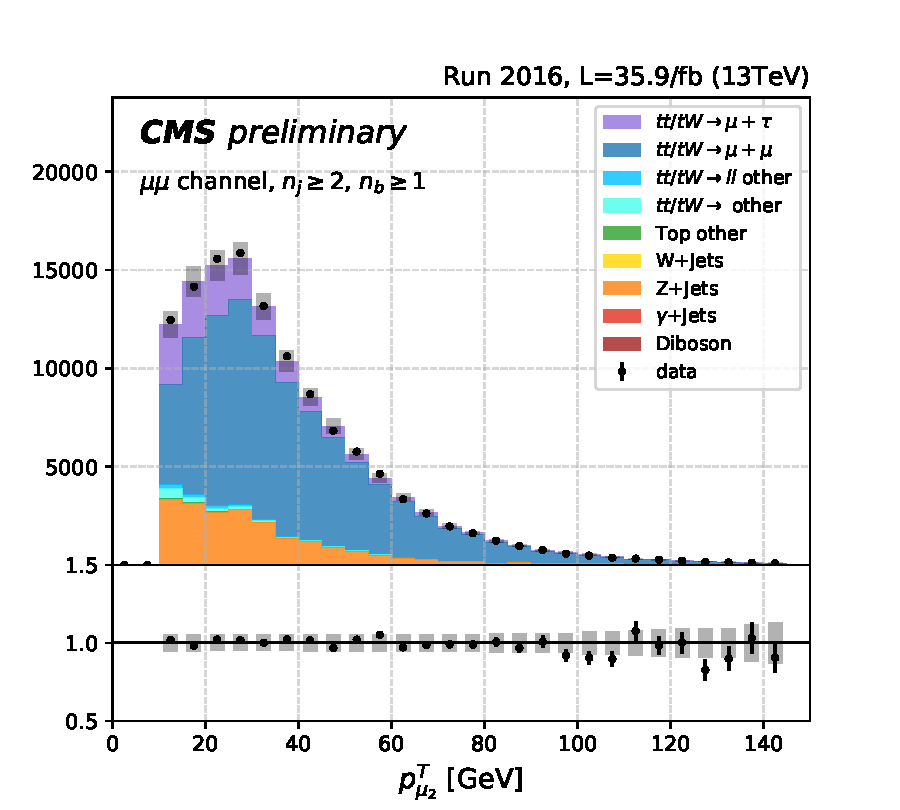
\includegraphics[width=0.49\textwidth]{chapters/Analysis/sectionPlots/figures/kinematics_pickles/mumu/12b/mumu_2b_lepton2_pt.pdf}
  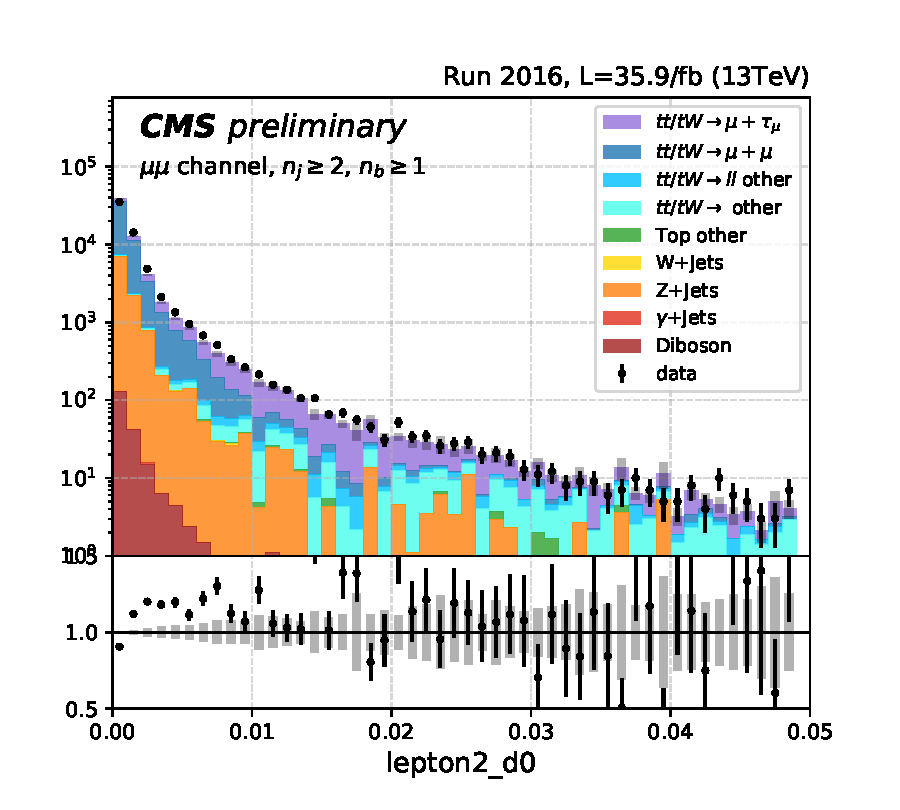
\includegraphics[width=0.49\textwidth]{chapters/Analysis/sectionSelection/figures/sob/mumu_lepton2_d0_logscale.pdf}
  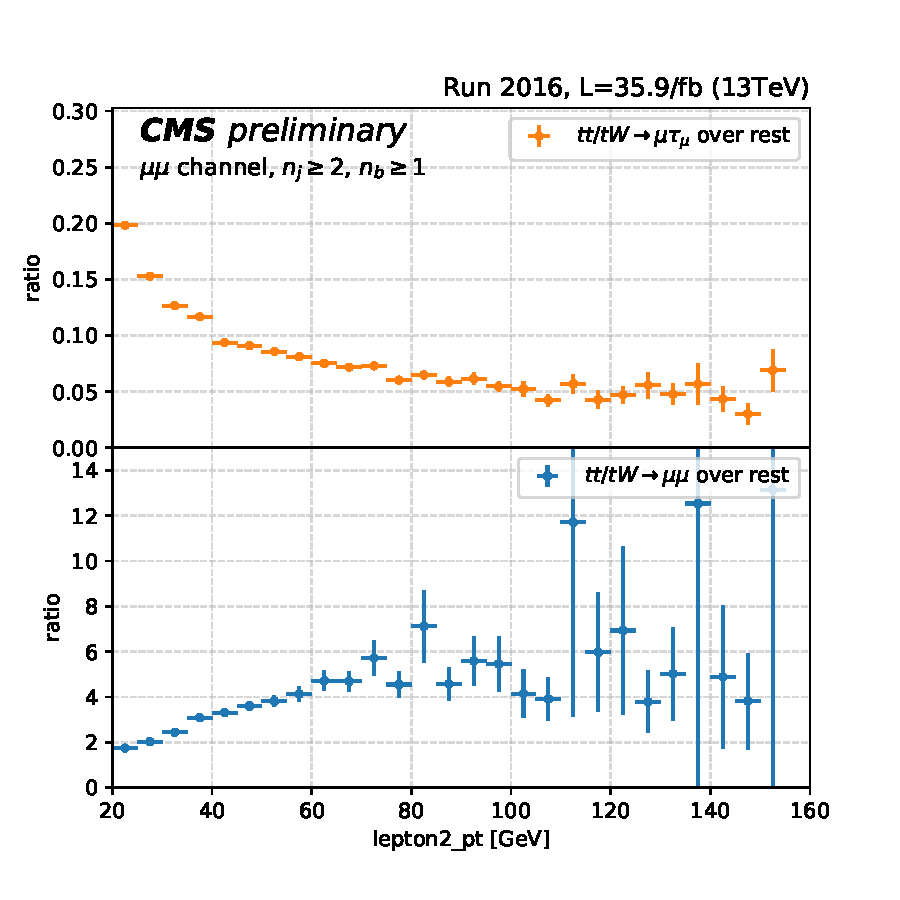
\includegraphics[width=0.49\textwidth]{chapters/Analysis/sectionSelection/figures/sob/mumu_lepton2_pt_2.pdf} 
  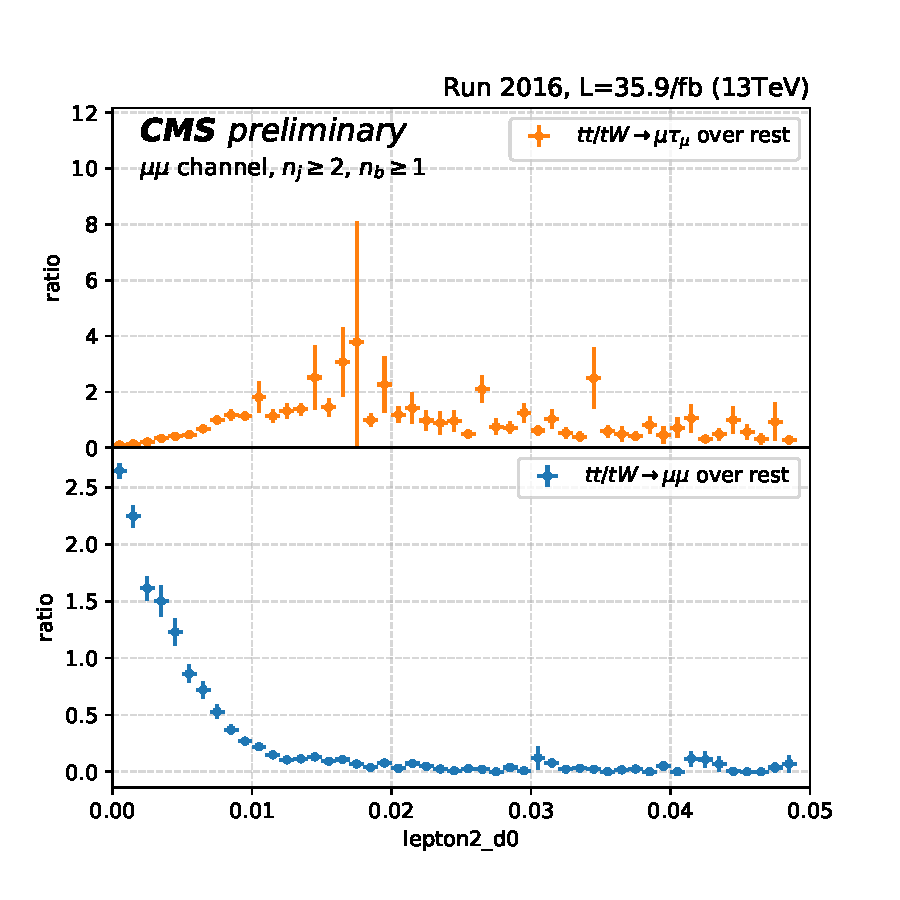
\includegraphics[width=0.49\textwidth]{chapters/Analysis/sectionSelection/figures/sob/mumu_lepton2_d0_2.pdf} 
  \caption{The distributions of the tailing muon \pt (\emph{upper left}) and impact parameter (\emph{upper right}). The ratios between $\ttbar/\tW \to \PGm \PGt \to \PGm \PGm$ and other simulations are shown as orange dots, while the ratios between $\ttbar/\tW \to \PGm \PGm$ and other simulations are shown as blue dots, as function of the tailing muon \pt (\emph{lower left}) and impact parameter (\emph{lower right}).
  \label{fig:analysis:selection:sob_mumu_lep2_pt}}
\end{figure}


% ----MARK finetuning ---
\subsubsection{Trigger Status of Dilepton Events} 
In dilepton channels \cee, \cmm, \cem, \cme, at least one of leading and trailing lepton is required to pass the single lepton trigger. A trigger test study is conducted to understand the proportions of events with both leptons firing, only leading lepton firing, and only trailing lepton firing. Figure~\ref{fig:analysis:selection:trTest} shows the proportions as function of the trailing lepton \pt in the \cmm, \cee, \cme, \cem channel. This is done by matching the leading and trailing lepton to the save triggering objects of single muon or electron HLT. 

\begin{figure}[h]
  \centering
  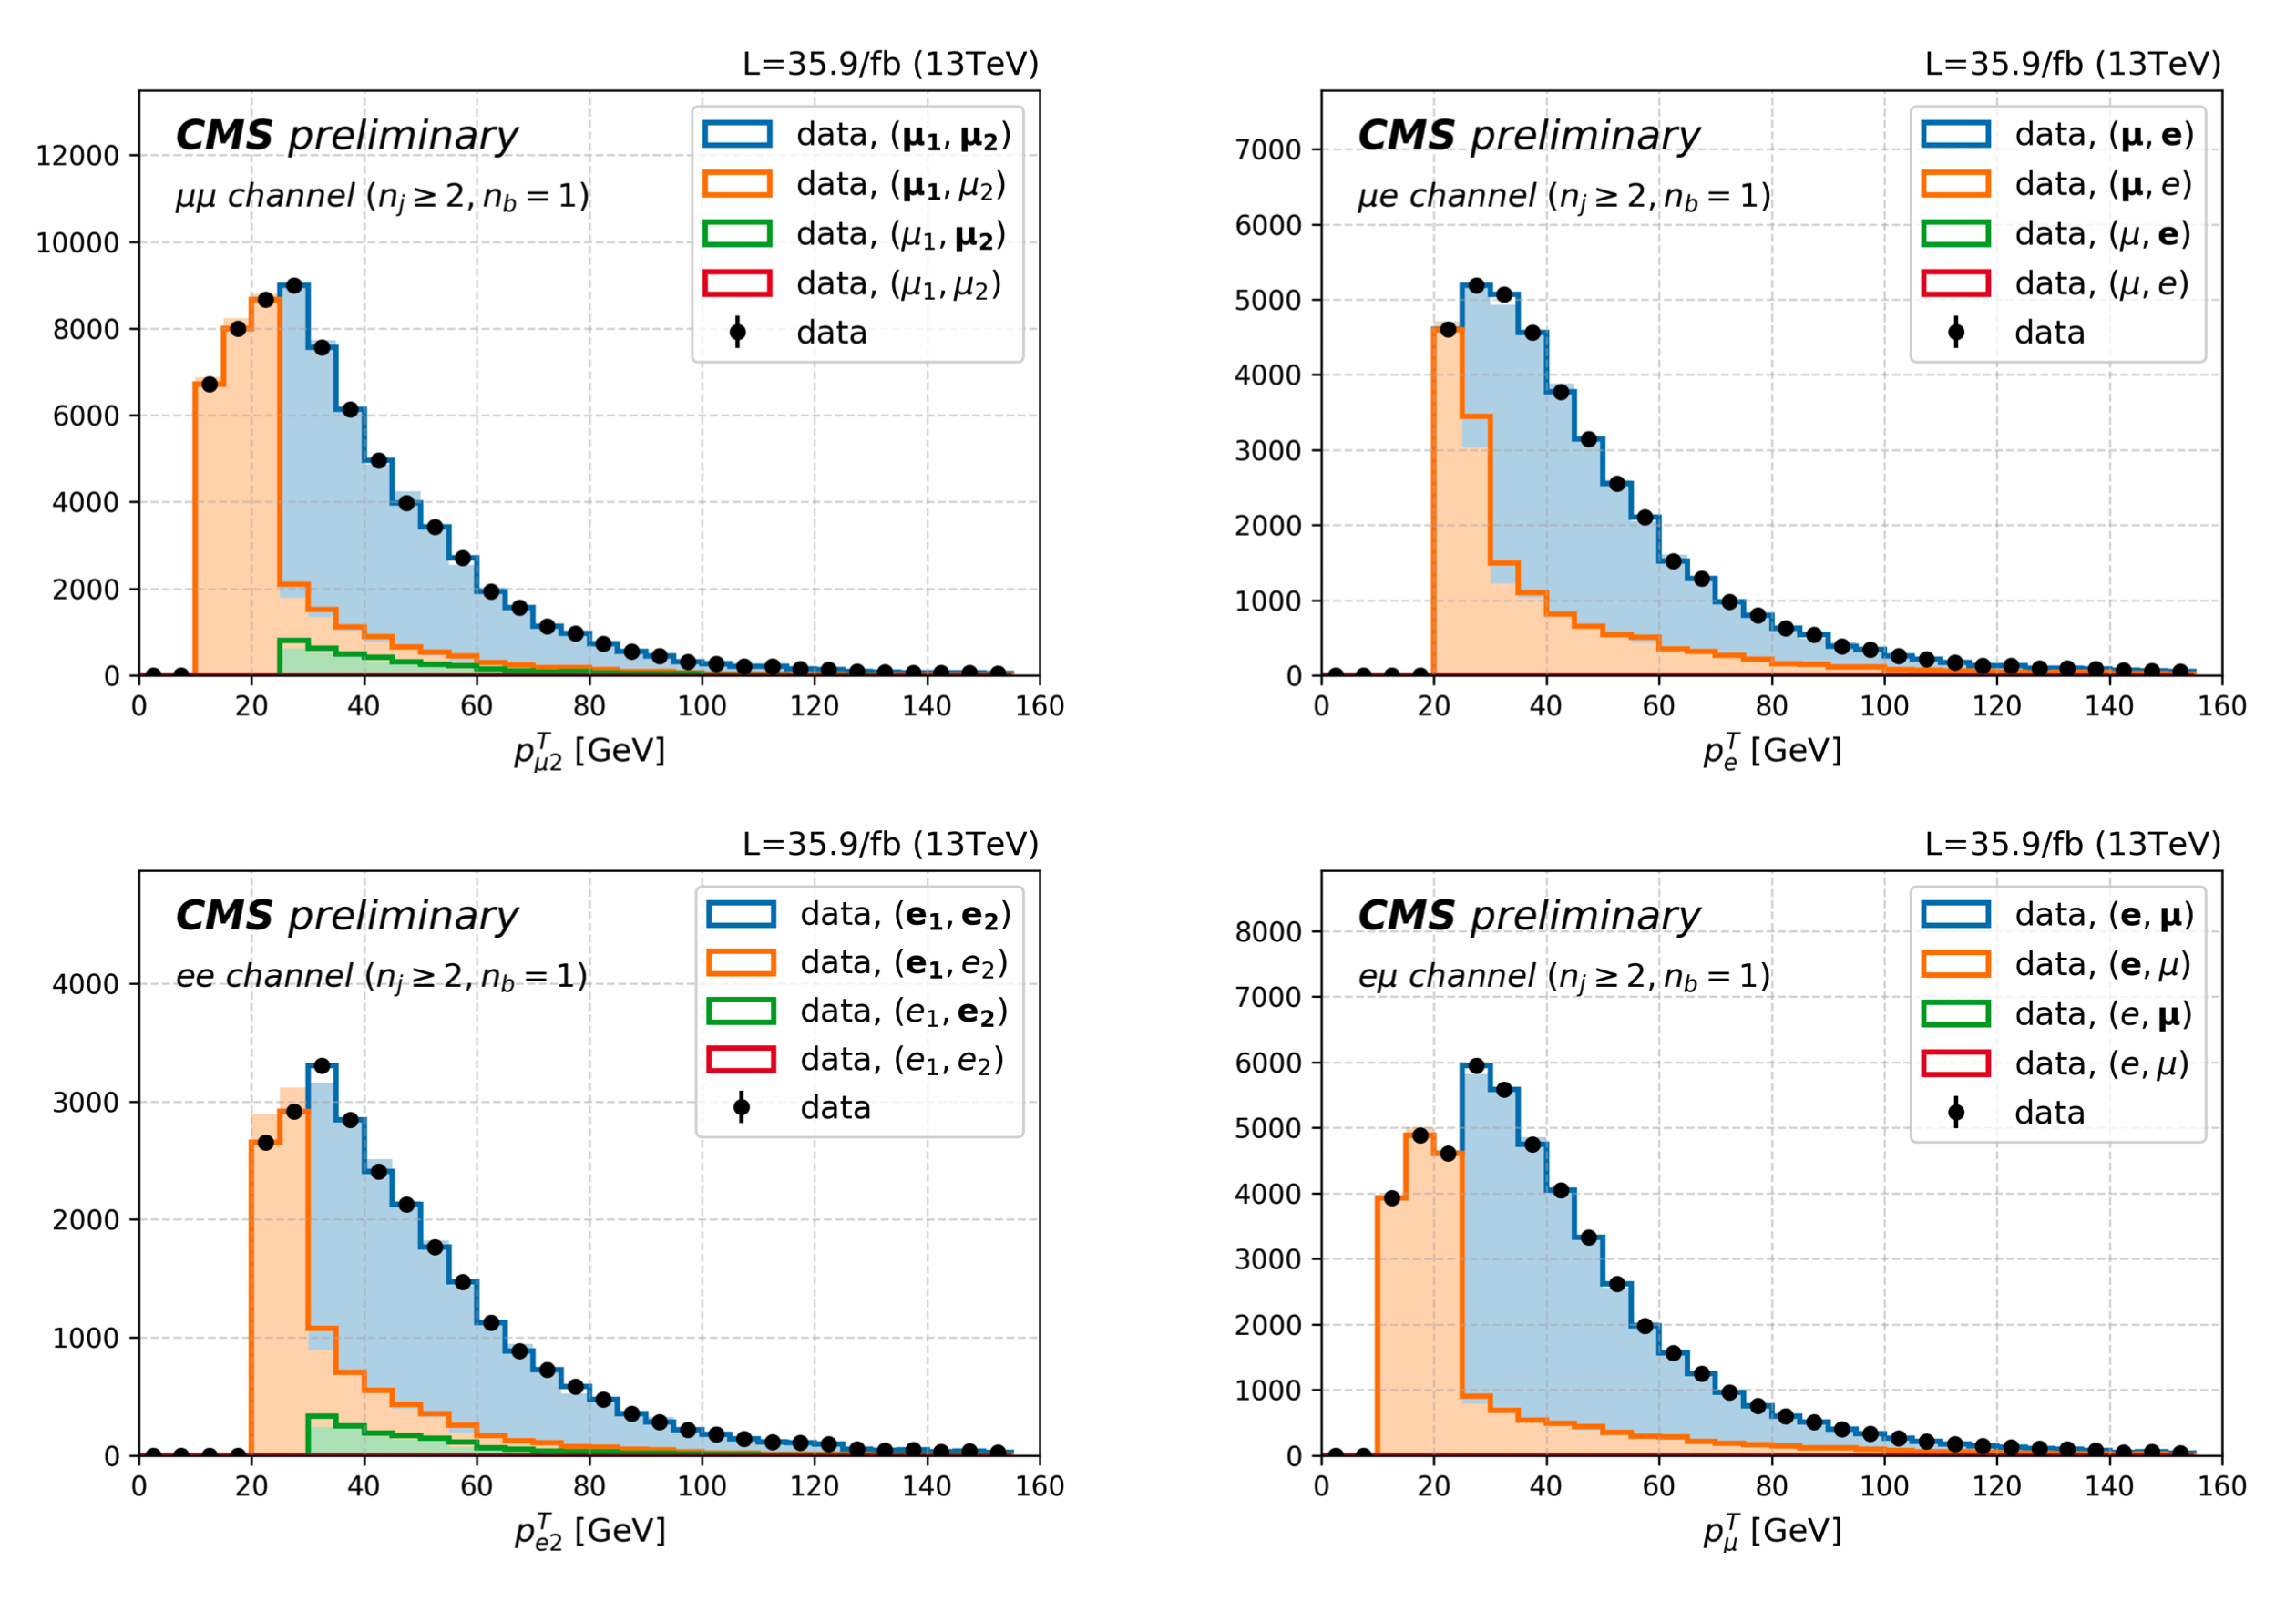
\includegraphics[width=0.99\textwidth]{chapters/Analysis/sectionSelection/figures/trTest.png}
  \caption{trailing lepton \pt in the \cmm,\cee,\cme,\cem channel. Data and MC events channel are split based on the trigger test of leading and trailing lepton: blue for both leptons firing trigger, orange for only leading lepton firing trigger, green for only trailing lepton firing trigger, red for neither leptons firing trigger.
  \label{fig:analysis:selection:trTest}}
\end{figure}






 

 
 
 
 







% Events are split based on the trigger test of the leading and trailing lepton, which has four possible scenarios, both pass (blue), only leading pass (orange), only trailing pass (green), both fail (red). But the case of both fail should not appear due the event selection requirement. The scenario needs attention is only the trailing lepton triggering the event. Since the shape analysis template fits the trailing lepton \pt in the dilepton channel, it is good to know the contributions from such scenario and decide whether extra treatment of trigger systematics is needed.









% \begin{table}[ht]
	\centering
	\setlength{\tabcolsep}{0.4em}
    \renewcommand{\arraystretch}{1.5}
    \small
    
    \begin{tabular}{|cc|cc|cc|cc|}
    
    %%%%%%%%%%%%%%%%%%
	% mu-trigger
	%%%%%%%%%%%%%%%%%%
    \multicolumn{8}{c}{single muon trigger} \\
    \hline
    \multicolumn{2}{|c|}{$\mu e$} 					& \multicolumn{2}{c|}{$\mu\mu$} 				  & \multicolumn{2}{c|}{$\mu \tau$} 					& \multicolumn{2}{c|}{$\mu + jets$} 			  	\\
    \hline
    1b & 2b                   						& 1b & 2b        	 						      & 1b & 2b        										& 1b & 2b         			        				\\
    \hline 
    \multicolumn{2}{|c|}{$n_{e,\mu,\tau_h} = 1,1,0$}& \multicolumn{2}{c|}{$n_{e,\mu,\tau_h} = 0,2,0$} & \multicolumn{2}{c|}{$n_{e,\mu,\tau_h} = 0,1,1$}      & \multicolumn{2}{c|}{$n_{e,\mu,\tau_h} = 0,1,0$} 	\\
    \multicolumn{2}{|c|}{$p^T_\mu,p^T_e>25,15$ GeV} & \multicolumn{2}{c|}{$p^T_\mu,p^T_\mu>25,10$ GeV}& \multicolumn{2}{c|}{$p^T_\mu,p^T_{\tau_h}>30,20$ GeV}& \multicolumn{2}{c|}{$p^T_\mu>30$ GeV}           	\\
    \multicolumn{2}{|c|}{$p^T_\mu>p^T_e$} 			& \multicolumn{2}{c|}{$|m_{\mu\mu}-m_Z|>15$ GeV } & \multicolumn{2}{c|}{ --- }						     & \multicolumn{2}{c|}{ --- } 						\\
    \multicolumn{2}{|c|}{$n_{jet}\geq2$}			& \multicolumn{2}{c|}{$n_{jet}\geq2$}             &  \multicolumn{2}{c|}{$n_{jet}\geq2$} 				 & \multicolumn{2}{c|}{$n_{jet}\geq4$}             	\\
    \hline

    
    %\multicolumn{8}{c}{} \\
    \multicolumn{8}{c}{single electron trigger} \\
    
    %%%%%%%%%%%%%%%%%%
	% e-trigger
	%%%%%%%%%%%%%%%%%%
    \hline
    \multicolumn{2}{|c|}{$e e$} 					& \multicolumn{2}{c|}{$e \mu$} 				      & \multicolumn{2}{c|}{$e \tau$} 			     		& \multicolumn{2}{c|}{$e + jets$} 			     	\\
    \hline
    1b & 2b                   						& 1b & 2b        	 						      & 1b & 2b        										& 1b & 2b         			        				\\
    \hline 
    \multicolumn{2}{|c|}{$n_{e,\mu,\tau_h} = 2,0,0$}& \multicolumn{2}{c|}{$n_{e,\mu,\tau_h} = 1,1,0$} & \multicolumn{2}{c|}{$n_{e,\mu,\tau_h} = 1,0,1$}      & \multicolumn{2}{c|}{$n_{e,\mu,\tau_h} = 1,0,0$} 	\\
    \multicolumn{2}{|c|}{$p^T_e,p^T_e>30,15$ GeV}   & \multicolumn{2}{c|}{$p^T_e,p^T_\mu>30,10$ GeV}  & \multicolumn{2}{c|}{$p^T_e,p^T_{\tau_h}>30,20$ GeV}  & \multicolumn{2}{c|}{$p^T_e>30$ GeV}           	\\
    \multicolumn{2}{|c|}{$|m_{ee}-m_Z|>15$ GeV }    & \multicolumn{2}{c|}{$p^T_e>p^T_\mu$}   		  & \multicolumn{2}{c|}{ --- }						     & \multicolumn{2}{c|}{ --- } 						\\
    \multicolumn{2}{|c|}{$n_{jet}\geq2$}			& \multicolumn{2}{c|}{$n_{jet}\geq2$}             & \multicolumn{2}{c|}{$n_{jet}\geq2$} 				 & \multicolumn{2}{c|}{$n_{jet}\geq4$}             	\\
    \hline
    
    \end{tabular}
    
    \caption{Analysis selections of 8 channels based on single muon and single electron triggers.}
    \label{tab:slt:eventSelection}
\end{table}





\begin{sidewaystable}[ht]
    \centering
    \setlength{\tabcolsep}{0.4em}
    \renewcommand{\arraystretch}{1.5}

    \caption{Composition of accepted $t\bar{t}$+$tW$ events, breakdown by 21 WW decay.  Values are in percent.}
    \resizebox{\textwidth}{!}{
    \begin{tabular}{|l|cc|cc|cc|cc|cc|cc|cc|cc|}
    
    
    \hline
    channel & \multicolumn{2}{|c|}{$\mu e$} & \multicolumn{2}{c|}{$\mu\mu$} & \multicolumn{2}{|c|}{$\mu \tau$} & \multicolumn{2}{|c|}{$\mu$+jets} & \multicolumn{2}{|c|}{$ee$} & \multicolumn{2}{|c|}{$e\mu$} & \multicolumn{2}{|c|}{$e \tau$} & \multicolumn{2}{|c|}{$e+jets$} \\
    \hline
    $\rm n_{b tag}$ & $n_b=1$ & $n_b\geq2$ & $n_b=1$ & $n_b\geq2$ & $n_b=1$ & $n_b\geq2$ & $n_b=1$ & $n_b\geq2$ & $n_b=1$ & $n_b\geq2$ & $n_b=1$ & $n_b\geq2$ & $n_b=1$ & $n_b\geq2$ & $n_b=1$ & $n_b\geq2$ \\ 
    \hline
    
    $tt/tW \to ee$                     &   -- &   -- &   -- &   -- &   -- &   -- &   -- &   -- & 87.4 & 87.8 &   -- &   -- &  0.7 &   -- &  3.1 &  3.1 \\ 
    $tt/tW \to \mu\mu$                 &   -- &   -- & 81.6 & 83.0 &   -- &   -- &  1.3 &  1.2 &   -- &   -- &   -- &   -- &   -- &   -- &   -- &   -- \\ 
    $tt/tW \to e\mu$                   & 86.5 & 87.0 &   -- &   -- &  0.8 &  0.5 &  3.3 &  3.3 &   -- &   -- & 82.7 & 84.1 &   -- &   -- &  1.4 &  1.4 \\ 
    $tt/tW \to \tau_{e}\tau_{e}$       &   -- &   -- &   -- &   -- &   -- &   -- &   -- &   -- &   -- &   -- &   -- &   -- &   -- &   -- &   -- &   -- \\ 
    $tt/tW \to \tau_{\mu}\tau_{\mu}$   &   -- &   -- &  0.7 &  0.6 &   -- &   -- &   -- &   -- &   -- &   -- &   -- &   -- &   -- &   -- &   -- &   -- \\ 
    $tt/tW \to \tau_{e}\tau_{\mu}$     &   -- &   -- &   -- &   -- &   -- &   -- &   -- &   -- &   -- &   -- &  0.6 &  0.6 &   -- &   -- &   -- &   -- \\ 
    $tt/tW \to \tau_{e}\tau_{h}$       &   -- &   -- &   -- &   -- &   -- &   -- &   -- &   -- &   -- &   -- &   -- &   -- &  3.1 &  3.2 &   -- &   -- \\ 
    $tt/tW \to \tau_{\mu}\tau_{h}$     &   -- &   -- &   -- &   -- &  3.2 &  3.6 &   -- &   -- &   -- &   -- &   -- &   -- &   -- &   -- &   -- &   -- \\ 
    $tt/tW \to \tau_{h}\tau_{h}$       &   -- &   -- &   -- &   -- &   -- &   -- &   -- &   -- &   -- &   -- &   -- &   -- &   -- &   -- &   -- &   -- \\ 
    $tt/tW \to e\tau_{e}$              &   -- &   -- &   -- &   -- &   -- &   -- &   -- &   -- & 11.7 & 11.5 &   -- &   -- &   -- &   -- &  0.8 &  0.8 \\ 
    $tt/tW \to e\tau_{\mu}$            &  4.1 &  4.0 &   -- &   -- &   -- &   -- &   -- &   -- &   -- &   -- & 11.2 & 11.0 &   -- &   -- &   -- &   -- \\ 
    $tt/tW \to e\tau_{h}$              &   -- &   -- &   -- &   -- &   -- &   -- &   -- &   -- &   -- &   -- &   -- &   -- & 57.5 & 63.6 &  3.4 &  3.6 \\ 
    $tt/tW \to \mu\tau_{e}$            &  8.3 &  8.2 &   -- &   -- &   -- &   -- &  0.6 &  0.7 &   -- &   -- &  3.6 &  3.6 &   -- &   -- &   -- &   -- \\ 
    $tt/tW \to \mu\tau_{\mu}$          &   -- &   -- & 15.7 & 15.8 &   -- &   -- &   -- &   -- &   -- &   -- &   -- &   -- &   -- &   -- &   -- &   -- \\ 
    $tt/tW \to \mu\tau_{h}$            &   -- &   -- &   -- &   -- & 57.4 & 63.6 &  3.4 &  3.6 &   -- &   -- &   -- &   -- &   -- &   -- &   -- &   -- \\ 
    $tt/tW \to eh$                     &   -- &   -- &   -- &   -- &   -- &   -- &   -- &   -- &   -- &   -- &  1.6 &   -- & 35.9 & 30.5 & 85.6 & 85.4 \\ 
    $tt/tW \to \mu h$                  &   -- &   -- &  1.7 &  0.5 & 35.7 & 30.1 & 85.3 & 85.3 &   -- &   -- &   -- &   -- &   -- &   -- &   -- &   -- \\ 
    $tt/tW \to \tau_{e}h$              &   -- &   -- &   -- &   -- &   -- &   -- &   -- &   -- &   -- &   -- &   -- &   -- &  1.9 &  1.6 &  4.8 &  4.7 \\ 
    $tt/tW \to \tau_{\mu}h$            &   -- &   -- &   -- &   -- &  2.1 &  1.6 &  5.0 &  4.9 &   -- &   -- &   -- &   -- &   -- &   -- &   -- &   -- \\ 
    $tt/tW \to \tau_{h}h$              &   -- &   -- &   -- &   -- &   -- &   -- &   -- &   -- &   -- &   -- &   -- &   -- &   -- &   -- &   -- &   -- \\ 
    $tt/tW \to hh$                     &   -- &   -- &   -- &   -- &   -- &   -- &   -- &   -- &   -- &   -- &   -- &   -- &   -- &   -- &   -- &   -- \\ 

    \hline
    \end{tabular}}
    \label{tab:analysis:selection:signal_breakdown}
    
\end{sidewaystable}

\begin{sidewaystable}
    \centering
    \setlength{\tabcolsep}{0.2em}
    \renewcommand{\arraystretch}{1.5}
    
    \caption{Estimates of the yields for various processes in the $ee$,
    $\mu\mu$, $e\mu$ and semileptonic final states broken down by the
    number of b tags.  The estimate of the expected yield is compared to
    the yield observed from data.  Uncertainties are statistical plus
    variation from luminosity and normalization uncertainties.}
    
    
    \resizebox{\textwidth}{!}{
        \begin{tabular}{l|ccccccc|cc}
        \hline
                                           & QCD                  & Diboson (non-WW)   & WW                 & Z                      & W & tW                   & $\rm t\bar{t}$         & Expected               & Observed \\
        \hline
        \multicolumn{10}{l}{$ee$}         \\
        \hline
        $N_{j} \geq 2, N_{b} = 0$          & --                   & $1014.2 \pm 104.7$ & $804.9 \pm 46.8$   & $55026.7 \pm 5713.1$   & $175.2 \pm 25.0$     & $854.4 \pm 58.0$     & $10865.1 \pm 609.1$    & $68740.4 \pm 5747.0$   & $68657$  \\
        $N_{j} \geq 2, N_{b} = 1$          & --                   & $119.6 \pm 12.4$   & $51.2 \pm 4.3$     & $5207.9 \pm 579.0$     & $10.1 \pm 4.8$       & $1415.3 \pm 89.8$    & $24815.2 \pm 1388.9$   & $31619.1 \pm 1507.5$   & $30332$  \\
        $N_{j} \geq 2, N_{b} \geq 2$       & --                   & $17.2 \pm 1.8$     & $3.3 \pm 0.8$      & $504.9 \pm 86.2$       & $5.2 \pm 3.7$        & $384.5 \pm 30.8$     & $14121.1 \pm 791.1$    & $15036.2 \pm 796.4$    & $14646$  \\
        \hline
        \multicolumn{10}{l}{$\mu\mu$}     \\
        \hline
        $N_{j} \geq 2, N_{b} = 0$          & --                   & $2628.2 \pm 271.0$ & $1944.1 \pm 110.6$ & $194725.6 \pm 20123.0$ & $455.9 \pm 43.1$     & $2081.2 \pm 127.6$   & $28399.5 \pm 1589.3$   & $230234.5 \pm 20188.2$ & $238485$ \\
        $N_{j} \geq 2, N_{b} = 1$          & --                   & $324.9 \pm 33.6$   & $128.4 \pm 8.9$    & $19150.5 \pm 2023.9$   & $80.0 \pm 16.4$      & $3469.2 \pm 205.5$   & $64582.6 \pm 3612.0$   & $87735.6 \pm 4145.7$   & $86354$  \\
        $N_{j} \geq 2, N_{b} \geq 2$       & --                   & $48.3 \pm 5.0$     & $5.8 \pm 1.1$      & $2028.9 \pm 253.5$     & $5.3 \pm 3.8$        & $976.6 \pm 65.4$     & $36916.5 \pm 2065.4$   & $39981.3 \pm 2082.0$   & $40011$  \\
        \hline
        \multicolumn{10}{l}{$e\mu$}         \\
        \hline
        $N_{j} = 0, N_{b} = 0$       & $4264.9 \pm 285.7$ & $748.9 \pm 77.6$ & $17566.8 \pm 983.8$ & $49838.9 \pm 5152.2$ & $3713.1 \pm 262.4$ & $3305.7 \pm 196.0$ & $9606.0 \pm 538.7$   & $89044.3 \pm 5291.3$ & $90784$  \\
        $N_{j} = 1, N_{b} = 0$       & $1907.5 \pm 164.2$ & $774.1 \pm 80.2$ & $7384.9 \pm 414.6$  & $13584.5 \pm 1424.6$ & $1700.9 \pm 131.7$ & $5413.8 \pm 313.9$ & $25755.0 \pm 1441.5$ & $56520.8 \pm 2104.4$ & $55427$  \\
        $N_{j} = 1, N_{b} = 1$       & $279.7 \pm 42.4$   & $21.2 \pm 2.5$   & $173.9 \pm 11.4$    & $712.9 \pm 98.8$     & $95.5 \pm 18.5$    & $6330.4 \pm 365.2$ & $32341.1 \pm 1809.6$ & $39954.7 \pm 1849.4$ & $39021$  \\
        $N_{j} \geq 2, N_{b} = 0$    & $737.0 \pm 95.6$   & $582.4 \pm 60.4$ & $2780.4 \pm 157.3$  & $5280.2 \pm 574.9$   & $710.3 \pm 60.7$   & $3117.8 \pm 185.5$ & $40246.2 \pm 2251.5$ & $53454.4 \pm 2340.0$ & $50301$  \\
        $N_{j} \geq 2, N_{b} = 1$    & $403.7 \pm 60.4$   & $47.0 \pm 5.2$   & $185.6 \pm 12.1$    & $605.3 \pm 89.0$     & $64.9 \pm 13.2$    & $5127.5 \pm 298.0$ & $91534.6 \pm 5118.7$ & $97968.5 \pm 5128.5$ & $93440$  \\
        $N_{j} \geq 2, N_{b} \geq 2$ & $203.0 \pm 29.2$   & $4.2 \pm 0.6$    & $13.1 \pm 1.8$      & $61.8 \pm 23.9$      & $14.7 \pm 6.1$     & $1510.7 \pm 95.4$  & $52401.6 \pm 2931.1$ & $54209.1 \pm 2932.9$ & $53859$  \\
        \hline
        \multicolumn{10}{l}{$e$ + jets}   \\
        \hline
        $N_{j} \geq 2, N_{b} = 1$          & $13189.3 \pm 740.4$  & $578.8 \pm 59.7$   & $65.2 \pm 5.2$     & $13637.7 \pm 1442.7$   & $46769.4 \pm 2637.7$ & $17675.4 \pm 999.7$  & $371951.7 \pm 20794.5$ & $463867.6 \pm 21047.6$ & $468222$ \\
        $N_{j} \geq 2, N_{b} \geq 2$       & $4665.8 \pm 263.9$   & $104.4 \pm 10.8$   & $7.1 \pm 1.3$      & $2367.0 \pm 279.5$     & $6359.5 \pm 378.1$   & $7591.6 \pm 435.9$   & $256643.9 \pm 14348.6$ & $277739.3 \pm 14365.3$ & $276116$ \\
        \hline
        \multicolumn{10}{l}{$\mu$ + jets} \\
        \hline
        $N_{j} \geq 2, N_{b} = 1$          & $42676.6 \pm 2389.3$ & $458.4 \pm 47.3$   & $90.1 \pm 6.7$     & $10504.3 \pm 1123.2$   & $71625.7 \pm 4028.2$ & $26161.6 \pm 1474.4$ & $572088.3 \pm 31982.5$ & $723605.0 \pm 32376.7$ & $710650$ \\
        $N_{j} \geq 2, N_{b} \geq 2$       & $13244.3 \pm 743.9$  & $82.9 \pm 8.6$     & $9.0 \pm 1.5$      & $1738.4 \pm 219.6$     & $9522.0 \pm 555.9$   & $11251.4 \pm 640.8$  & $397617.9 \pm 22229.3$ & $433465.8 \pm 22259.0$ & $429861$ \\
        \hline
    \end{tabular}}

    \label{tab:analysis:selection:yieldsShape1}
\end{sidewaystable}
\begin{sidewaystable}[]
    \centering
    \setlength{\tabcolsep}{0.4em}
    \renewcommand{\arraystretch}{1.5}
    
    \caption{Estimates of the yields for various processes in
    the $e\tau$ and $\mu\tau$ categories broken down by the number of b tags.
    The estimate of the expected yield is compared to the yield observed
    from data.  Uncertainties are statistical only.}
    
    \resizebox{\textwidth}{!}{
        \begin{tabular}{l|ccccccc|cc}
        \hline
                                        & QCD                  & Diboson (non-WW) & WW               & Z                      & W                    & tW                & $\sf t\bar{t}$     & Expected               & Observed \\
        \hline
        \multicolumn{10}{l}{$e\tau$}   \\
        \hline
        $N_{j} = 0, N_{b} = 0$          & $14609.7 \pm 843.7$  & $11.7 \pm 1.4$   & $102.2 \pm 7.2$  & $30670.4 \pm 3175.9$   & $9505.8 \pm 594.4$   & $11.1 \pm 3.7$    & $29.7 \pm 2.8$     & $54940.5 \pm 3339.4$   & $55591$  \\
        $N_{j} = 1, N_{b} = 0$          & $1512.7 \pm 125.2$   & $10.0 \pm 1.2$   & $20.9 \pm 2.3$   & $3237.1 \pm 355.2$     & $1159.9 \pm 98.0$    & $20.8 \pm 5.2$    & $76.3 \pm 5.7$     & $6037.5 \pm 389.2$     & $6074$   \\
        $N_{j} \geq 2, N_{b} = 0$       & $5519.7 \pm 363.2$   & $233.6 \pm 24.3$ & $269.8 \pm 16.8$ & $6721.8 \pm 724.1$     & $6906.0 \pm 410.6$   & $551.2 \pm 40.4$  & $5933.6 \pm 333.3$ & $26135.7 \pm 968.7$    & $25788$  \\
        $N_{j} = 1, N_{b} = 1$          & $789.5 \pm 77.4$     & $8.0 \pm 1.0$    & $16.4 \pm 2.0$   & $725.6 \pm 99.6$       & $650.5 \pm 60.3$     & $675.5 \pm 47.6$  & $3381.9 \pm 190.7$ & $6247.5 \pm 241.2$     & $6256$   \\
        $N_{j} = 2, N_{b} = 1$          & $421.6 \pm 59.9$     & $11.7 \pm 1.3$   & $10.8 \pm 1.6$   & $424.7 \pm 69.2$       & $305.0 \pm 33.4$     & $538.3 \pm 39.7$  & $5994.7 \pm 336.8$ & $7706.7 \pm 352.8$     & $7388$   \\
        $N_{j} \geq 3, N_{b} = 1$       & $315.4 \pm 56.0$     & $13.1 \pm 1.5$   & $5.0 \pm 1.0$    & $212.1 \pm 42.9$       & $169.3 \pm 23.1$     & $302.1 \pm 25.7$  & $6021.4 \pm 338.2$ & $7038.5 \pm 347.2$     & $6660$   \\
        $N_{j} = 2, N_{b} \geq 2$       & $48.4 \pm 16.4$      & $1.1 \pm 0.2$    & $0.3 \pm 0.2$    & $18.8 \pm 15.9$        & $10.6 \pm 5.8$       & $83.4 \pm 11.1$   & $2606.9 \pm 147.4$ & $2769.5 \pm 149.7$     & $2683$   \\
        $N_{j} \geq 3, N_{b} \geq 2$    & $81.3 \pm 28.8$      & $1.8 \pm 0.3$    & $0.3 \pm 0.2$    & $55.2 \pm 14.0$        & $18.0 \pm 6.9$       & $87.8 \pm 11.5$   & $3574.9 \pm 201.5$ & $3819.4 \pm 204.5$     & $3704$   \\
        \hline
        \multicolumn{10}{l}{$\mu\tau$} \\
        \hline
        $N_{j} = 0, N_{b} = 0$          & $19581.5 \pm 1133.6$ & $27.6 \pm 3.1$   & $244.6 \pm 15.3$ & $103926.9 \pm 10727.5$ & $20342.3 \pm 1205.2$ & $19.3 \pm 5.0$    & $66.2 \pm 5.1$     & $144208.5 \pm 10854.4$ & $146128$ \\
        $N_{j} = 1, N_{b} = 0$          & $2255.6 \pm 167.9$   & $24.0 \pm 2.6$   & $37.0 \pm 3.4$   & $8216.3 \pm 868.5$     & $2470.3 \pm 177.3$   & $33.8 \pm 6.8$    & $162.4 \pm 10.6$   & $13199.4 \pm 902.2$    & $13293$  \\
        $N_{j} \geq 2, N_{b} = 0$       & $5467.2 \pm 372.9$   & $313.5 \pm 32.5$ & $413.2 \pm 24.9$ & $10752.1 \pm 1139.7$   & $10989.1 \pm 640.3$  & $879.2 \pm 59.4$  & $9261.1 \pm 519.4$ & $38075.4 \pm 1457.1$   & $38184$  \\
        $N_{j} = 1, N_{b} = 1$          & $1452.3 \pm 113.6$   & $12.3 \pm 1.4$   & $27.8 \pm 2.8$   & $1632.3 \pm 193.8$     & $1199.1 \pm 96.4$    & $1112.9 \pm 72.6$ & $5266.7 \pm 296.1$ & $10703.3 \pm 390.8$    & $10628$  \\
        $N_{j} = 2, N_{b} = 1$          & $709.7 \pm 75.4$     & $17.6 \pm 1.9$   & $18.1 \pm 2.1$   & $708.4 \pm 101.7$      & $568.1 \pm 50.5$     & $769.3 \pm 53.1$  & $9493.5 \pm 532.4$ & $12284.6 \pm 552.1$    & $12048$  \\
        $N_{j} \geq 3, N_{b} = 1$       & $438.5 \pm 70.7$     & $19.5 \pm 2.1$   & $9.7 \pm 1.5$    & $384.5 \pm 62.6$       & $292.9 \pm 32.0$     & $480.7 \pm 36.5$  & $9413.5 \pm 527.9$ & $11039.3 \pm 538.5$    & $10314$  \\
        $N_{j} = 2, N_{b} \geq 2$       & $111.1 \pm 19.9$     & $1.7 \pm 0.2$    & $1.0 \pm 0.4$    & $58.6 \pm 23.6$        & $56.0 \pm 16.9$      & $153.8 \pm 16.5$  & $4157.7 \pm 234.1$ & $4539.9 \pm 237.3$     & $4321$   \\
        $N_{j} \geq 3, N_{b} \geq 2$    & $117.5 \pm 35.6$     & $3.0 \pm 0.4$    & $1.4 \pm 0.5$    & $79.4 \pm 22.2$        & $18.1 \pm 6.9$       & $157.9 \pm 16.7$  & $5599.2 \pm 314.7$ & $5976.5 \pm 318.0$     & $5705$   \\
        \hline
    \end{tabular}}

    \label{tab:analysis:selection:yieldsShape2}
\end{sidewaystable}





    \begin{tabular}{l|cccccccc|cc}
    \hline
        & QCD & VV  & $\gamma$ & Z & W & t & tW & tt & total & data      \\
    \hline
    
    $\mu e$, $n_b=1$                   &       --$\pm$     -- &     90.3$\pm$    4.2 &      0.9$\pm$    0.9 &    202.7$\pm$   37.6 &     13.4$\pm$    5.1 &      9.5$\pm$    2.6 &   2107.6$\pm$   53.1 &  38871.4$\pm$   87.5 &  41295.8$\pm$  109.2 &  41047.0$\pm$  202.6 \\ 
    $\mu e$, $n_b\geq2$                &       --$\pm$     -- &      5.9$\pm$    1.0 &       --$\pm$     -- &       --$\pm$     -- &      3.1$\pm$    2.2 &      2.3$\pm$    1.6 &    625.7$\pm$   28.9 &  22647.7$\pm$   66.8 &  23270.9$\pm$   74.1 &  23918.0$\pm$  154.7 \\ 
    \hline
    $\mu\mu$, $n_b=1$                  &       --$\pm$     -- &    370.4$\pm$    5.8 &      4.1$\pm$    1.8 &  18046.9$\pm$  455.4 &     52.4$\pm$   11.7 &     55.8$\pm$    6.7 &   3406.2$\pm$   68.8 &  62266.6$\pm$  112.4 &  84202.3$\pm$  474.3 &  84284.0$\pm$  290.3 \\ 
    $\mu\mu$, $n_b\geq2$               &       --$\pm$     -- &     45.8$\pm$    1.5 &      0.0$\pm$    0.0 &   1945.7$\pm$  142.0 &      3.6$\pm$    2.6 &      3.9$\pm$    1.8 &    959.3$\pm$   36.2 &  35685.2$\pm$   85.1 &  38643.4$\pm$  169.6 &  39253.0$\pm$  198.1 \\ 
    \hline
    $\mu\tau$, $n_b=1$                 &   1130.7$\pm$  108.8 &     52.3$\pm$    2.6 &     11.8$\pm$    3.2 &    866.7$\pm$   78.7 &    730.8$\pm$   42.9 &    182.6$\pm$   12.4 &   1291.0$\pm$   41.9 &  18430.0$\pm$   60.6 &  22695.9$\pm$  159.6 &  21621.0$\pm$  147.0 \\ 
    $\mu\tau$, $n_b\geq2$              &    346.6$\pm$   51.5 &      5.5$\pm$    0.7 &      0.9$\pm$    0.8 &    103.6$\pm$   29.6 &     56.9$\pm$   14.4 &     36.8$\pm$    5.6 &    322.6$\pm$   21.0 &   9647.6$\pm$   43.7 &  10520.4$\pm$   78.3 &   9934.0$\pm$   99.7 \\ 
    \hline
    $\mu$+jets, $n_b=1$                &  24300.4$\pm$ 3404.9 &    371.0$\pm$    5.2 &   1501.2$\pm$   67.5 &   7533.2$\pm$  265.9 &  49248.1$\pm$  327.3 &   8484.6$\pm$   85.3 &  24447.8$\pm$  187.0 & 514064.6$\pm$  327.2 & 629950.9$\pm$ 3453.3 & 630704.0$\pm$  794.2 \\ 
    $\mu$+jets, $n_b\geq2$             &   4650.7$\pm$ 1399.5 &     61.4$\pm$    2.0 &    248.3$\pm$   31.8 &   1331.9$\pm$  114.0 &   6524.2$\pm$  118.8 &   5172.2$\pm$   66.7 &  10335.6$\pm$  121.4 & 356185.1$\pm$  272.2 & 384509.5$\pm$ 1442.2 & 385397.0$\pm$  620.8 \\ 
    \hline
    $e e$, $n_b=1$                     &       --$\pm$     -- &    138.2$\pm$    3.6 &      2.8$\pm$    1.2 &   4726.5$\pm$  215.7 &      5.4$\pm$    2.8 &      1.1$\pm$    0.8 &   1382.0$\pm$   42.7 &  23447.3$\pm$   66.9 &  29703.3$\pm$  229.9 &  29491.0$\pm$  171.7 \\ 
    $e e$, $n_b\geq2$                  &       --$\pm$     -- &     16.2$\pm$    0.9 &      0.1$\pm$    0.1 &    500.5$\pm$   67.8 &      3.7$\pm$    2.6 &      2.1$\pm$    1.2 &    371.4$\pm$   22.1 &  13412.7$\pm$   50.7 &  14306.6$\pm$   87.5 &  14334.0$\pm$  119.7 \\ 
    \hline
    $e\mu$, $n_b=1$                    &       --$\pm$     -- &    127.2$\pm$    4.9 &     25.5$\pm$   13.2 &    411.9$\pm$   52.7 &     32.8$\pm$    7.2 &     37.6$\pm$    5.4 &   2917.6$\pm$   62.7 &  49878.6$\pm$   99.2 &  53431.1$\pm$  129.8 &  52362.0$\pm$  228.8 \\ 
    $e\mu$, $n_b\geq2$                 &       --$\pm$     -- &      9.0$\pm$    1.3 &      1.9$\pm$    1.1 &     59.0$\pm$   19.5 &      6.5$\pm$    3.2 &      6.1$\pm$    2.2 &    837.9$\pm$   33.8 &  28374.1$\pm$   74.9 &  29294.5$\pm$   84.6 &  29860.0$\pm$  172.8 \\ 
    \hline
    $e\tau$, $n_b=1$                   &    874.2$\pm$   90.3 &     38.0$\pm$    2.1 &    194.5$\pm$   38.8 &    677.8$\pm$   69.3 &    456.3$\pm$   32.9 &    125.3$\pm$   10.0 &    908.2$\pm$   34.6 &  12884.7$\pm$   49.7 &  16159.1$\pm$  139.0 &  15309.0$\pm$  123.7 \\ 
    $e\tau$, $n_b\geq2$                &     94.2$\pm$   46.3 &      3.0$\pm$    0.4 &     10.0$\pm$    2.9 &     53.4$\pm$   21.3 &     28.7$\pm$    8.5 &     43.4$\pm$    6.0 &    196.1$\pm$   15.9 &   6682.4$\pm$   35.8 &   7111.3$\pm$   65.1 &   7006.0$\pm$   83.7 \\ 
    \hline
    $e$+jets, $n_b=1$                  &  25625.1$\pm$ 2941.3 &    494.9$\pm$    5.1 &  12035.7$\pm$  173.0 &  13119.8$\pm$  323.2 &  34481.3$\pm$  266.1 &   5786.3$\pm$   68.8 &  17454.7$\pm$  154.8 & 360917.6$\pm$  268.5 & 469915.4$\pm$ 2992.9 & 464543.0$\pm$  681.6 \\ 
    $e$+jets, $n_b\geq2$               &   3327.4$\pm$ 1476.4 &     84.5$\pm$    2.0 &   2095.3$\pm$   78.4 &   2520.8$\pm$  138.5 &   4696.3$\pm$   98.0 &   3524.2$\pm$   53.7 &   7616.3$\pm$  102.3 & 249557.0$\pm$  223.4 & 273421.8$\pm$ 1509.3 & 274162.0$\pm$  523.6 \\ 
    \hline

    \end{tabular}

\FloatBarrier


